\chapter{Continuous Integration}
Continuous is geregeld door TravisCI, voor open source projecten is TravisCI gratis te gebruiken.
Omdat het project met Gradle is gebouwd is het makkelijk om CI ondersteuning toe te voegen aan de backend.
Het commando "gradle test" draait alle tests in het project, als er iets fout gaat is dit ook meteen in Github zichtbaar.
\linebreak
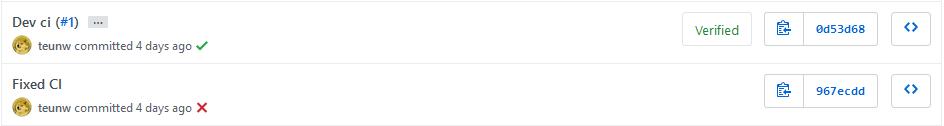
\includegraphics[width=\textwidth]{images/TravisCI.png}